\chapter{计划书}
\label{cha:intro}
计划书中包含目标阐述、关键问题、具体任务和具体方案。

\section{目标阐述}
红外遥控是利用近红外光进行数据传输的一种控制方式。
近红外光波长0.76um-1.5um,红外遥控收发器件波长一般为0.8um-0.94um,
具有传输效率高,成本低,电路实现简单,抗干扰强等特点,在家用电器上被广泛使用。
此处设计一个\textbf{红外发射接收器与红外接收器,
能够实现通过按按钮而发出不同的红外波段,以达到控制的功能。}


\section{关键问题}
1. 按按钮发出不一样的红外波段

2. 红外发射和接收稳定,不易受外界波段的干扰

3. 具有可移植接口,方便进一步开发 

\section{具体任务}
1. 通过开关控制阻值,以实现不同的射频

2. 加上滤波和放大,以减少外界波段的干扰

3. 采取模块化设计,留有接口

\section{具体方案和关键技术}
详细解释了选用的芯片和原理。

\subsection{NE555}
使用NE555产生红外光线。因为NE555时基电路(集成电路)性价比高,
且价格低廉,外围元件少,根据应用需要可设计不同功能,应用十分广泛。

由NE555芯片手册可知,\textbf{通过控制RA和RB的比例即可控制频率和占空比}。
\begin{figure}[H] % use float package if you want it here
  \centering
  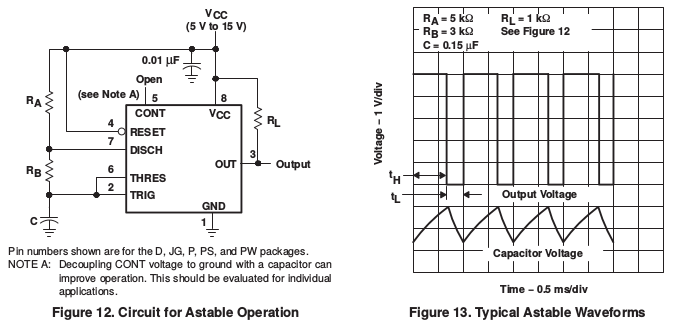
\includegraphics[width=0.8\textwidth]{1.png}
  \caption{NE555芯片手册}
  \label{fig:xfig1}
\end{figure}
比方说:使用NE555产生38kHz, 占空比为1/3的方波信号。

产生方波的频率 = 0.693((RA+2RB)*C) ,占空比 = RB/(RA+2RB)


因为红外发射管最佳的占空比是1/3,C一般为0.01uF,所以计算之后RA = RB =1.2k

此处,由于我们需要控制发射频率,因此我们把RA变成可调的电阻。

\subsection{光电二极管}
接收我们使用光电二极管用于接收产生的红外信号。
光电二极管是一种能够将光根据使用方式,转换成电流或者电压信号的光探测器。
管芯常使用一个具有光敏特征的PN结,对光的变化非常敏感,具有单向导电性,
而且光强不同的时候会改变电学特性,因此,可以\textbf{利用光照强弱来改变电路中的电流}。

\subsection{BC848B和2SC1815三极管}
使用此两款三极管以用于放大和解调。